\begin{figure} [htbp]
  \begin{subfigure}[b]{.49\textwidth}
   \centering
   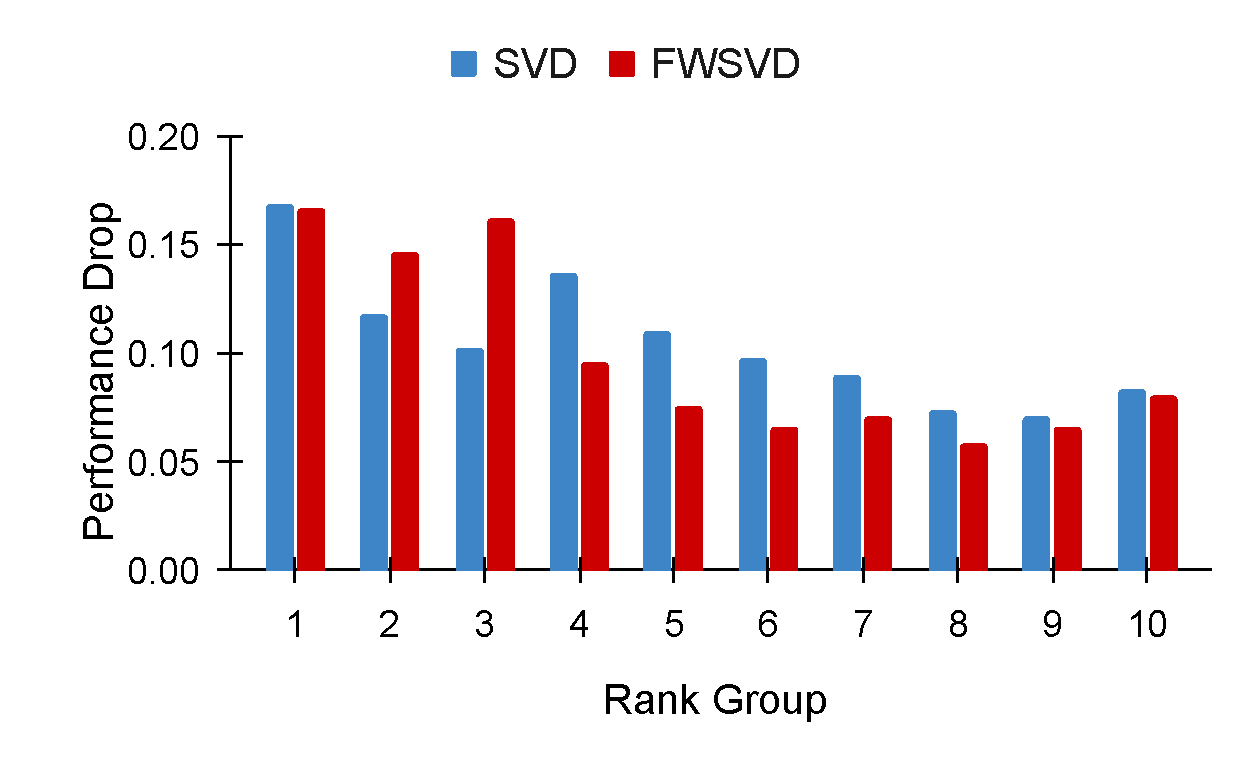
\includegraphics[width=\textwidth]{figures/app_mrpc_per.pdf}
       \caption{MRPC performance drop}
       \label{app:mrpc_per}
       \end{subfigure}
\begin{subfigure}[b]{.49\textwidth}
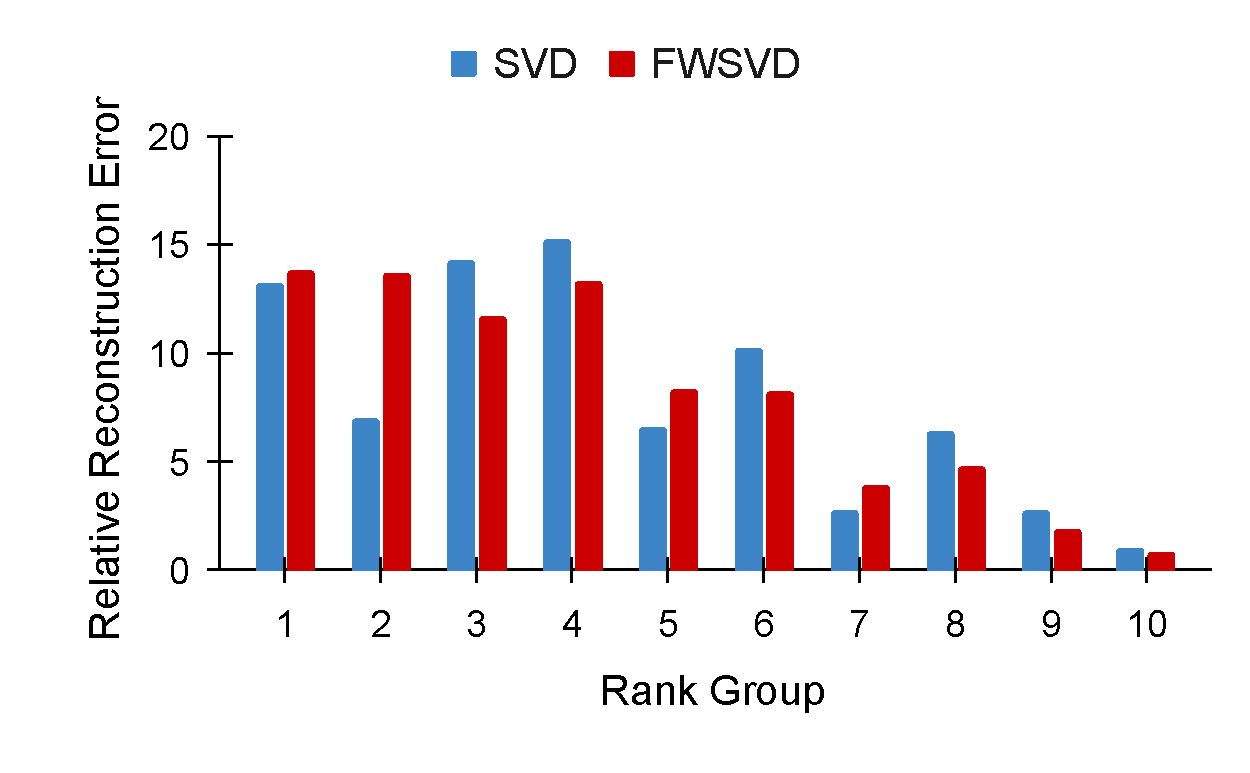
\includegraphics[width=\textwidth]{figures/app_mrpc_err.pdf}
\centering
  \caption{MRPC error}
   \label{app:mrpc_err}
\end{subfigure}
  \begin{subfigure}[b]{.49\textwidth}
   \centering
   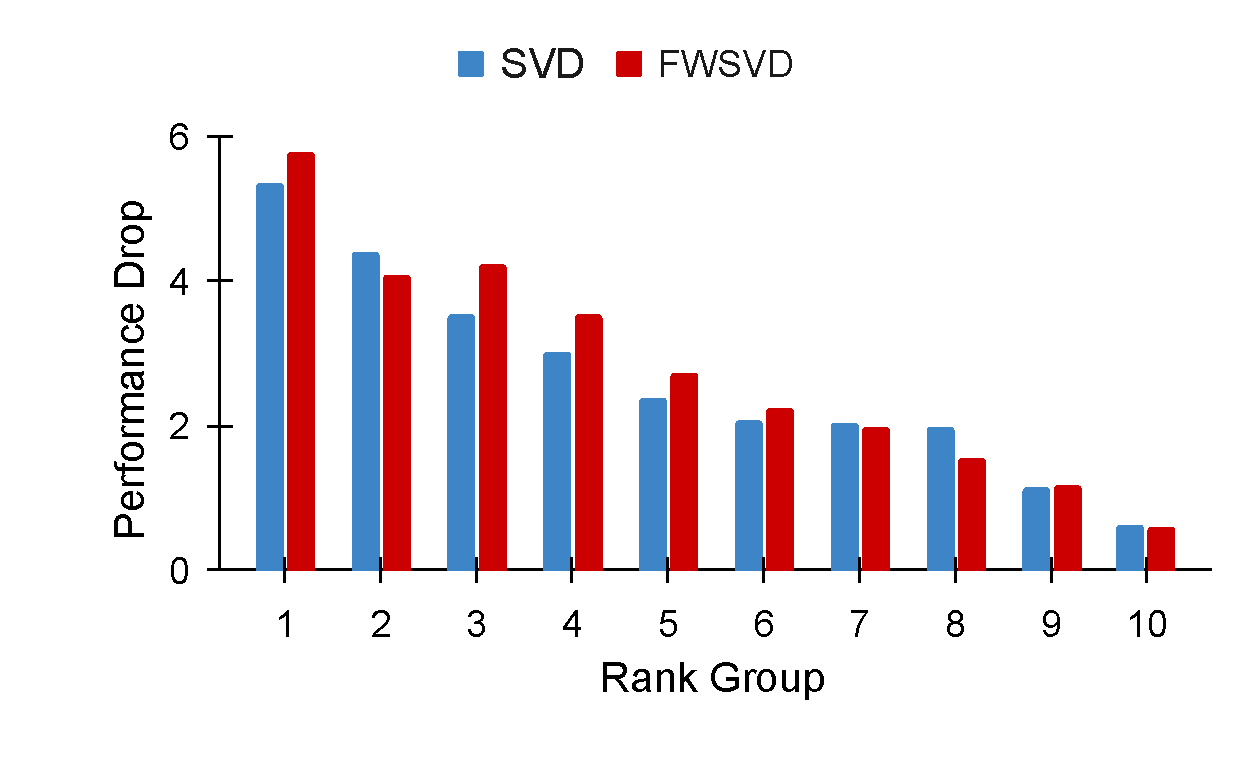
\includegraphics[width=\textwidth]{figures/app_ner_perpdf.pdf}
       \caption{CoNLL-03 performance Drop}
       \label{app:ner_per}
       \end{subfigure}
\begin{subfigure}[b]{.49\textwidth}
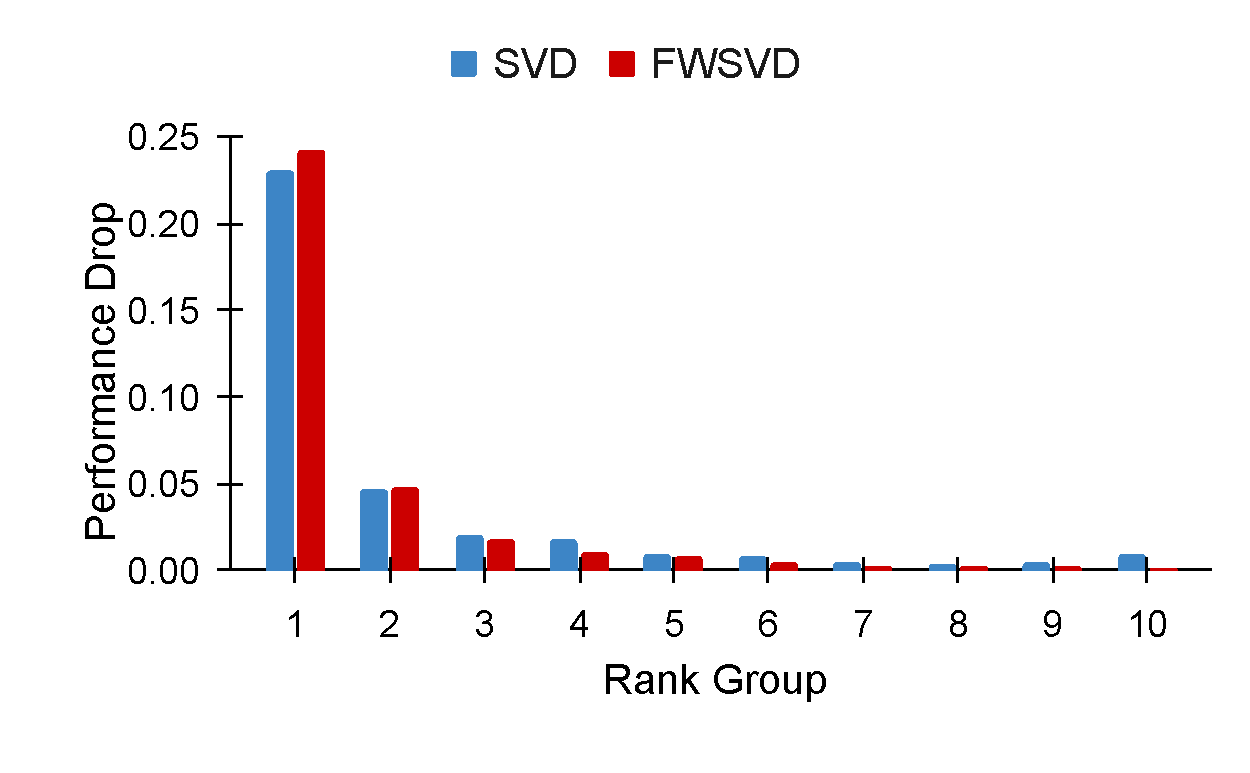
\includegraphics[width=\textwidth]{figures/app_ner_err.pdf}
\centering
  \caption{CoNLL-03 Error}
   \label{app:ner_err}
\end{subfigure}
  \begin{subfigure}[b]{.49\textwidth}
   \centering
   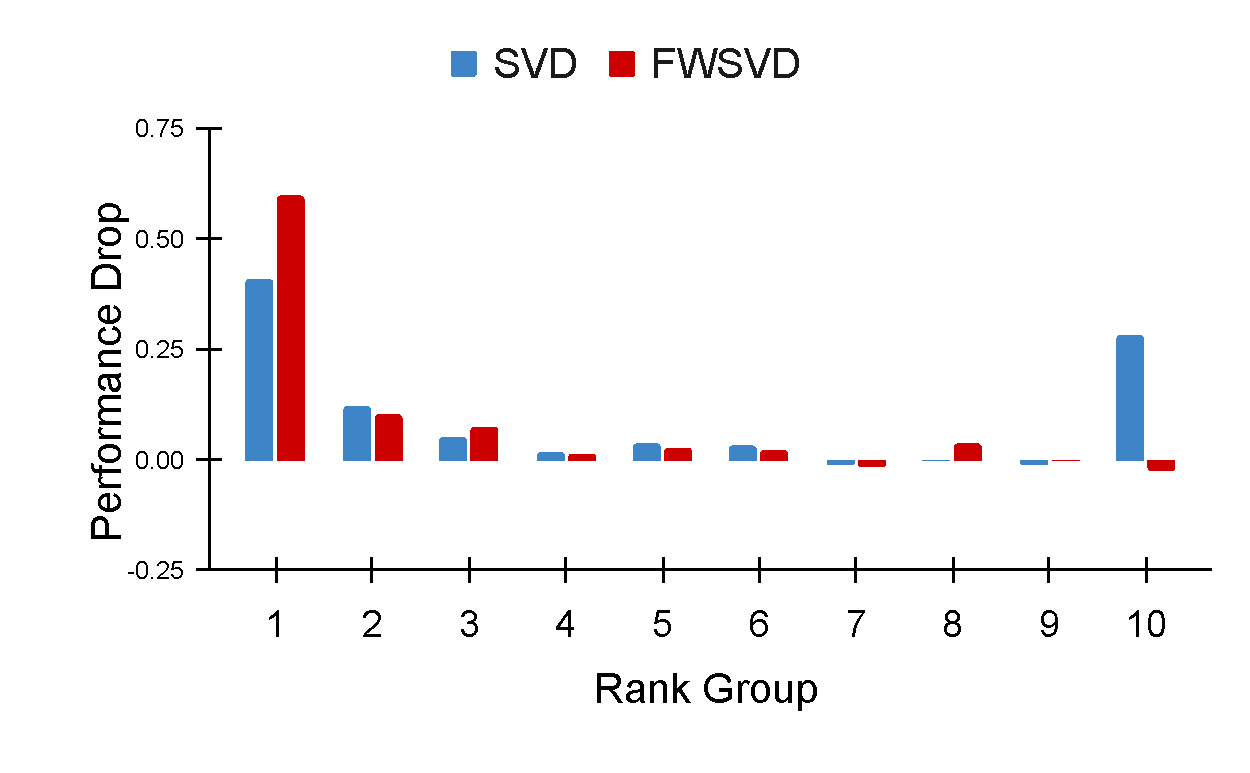
\includegraphics[width=\textwidth]{figures/app_cola_per.pdf}
       \caption{COLA performance drop}
       \label{app:cola_per}
       \end{subfigure}
\begin{subfigure}[b]{.49\textwidth}
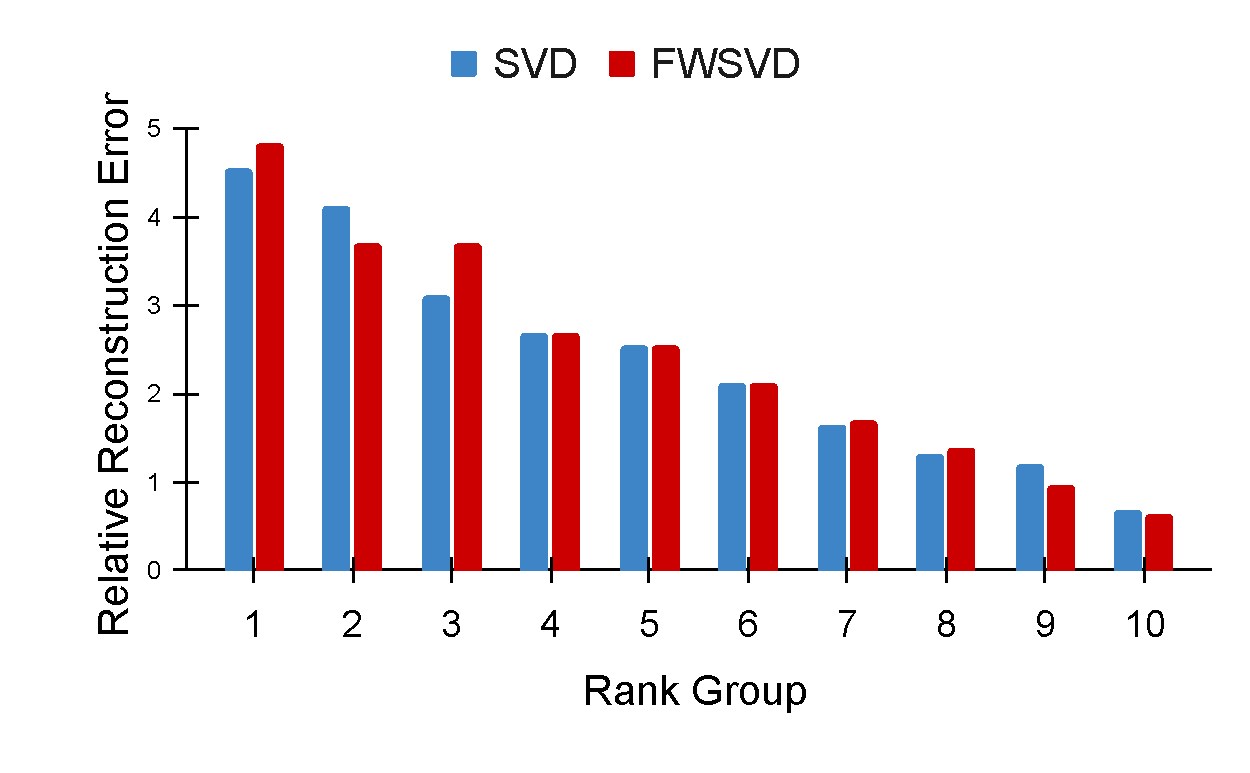
\includegraphics[width=\textwidth]{figures/app_cola_err.pdf}
\centering
  \caption{CoLA Error}
   \label{app:cola_err}
\end{subfigure}
\caption{The empirical evidence of mismatched objectives between  a standard low-rank factorization and task performance.
}
\label{app:err_per}
\end{figure}